% -*- Mode:TeX -*-
% LaTeX template for CinC papers                   v 1.1a 22 August 2010
%
% To use this template successfully, you must have downloaded and unpacked:
%       http://www.cinc.org/authors_kit/papers/latex.tar.gz
% or the same package in zip format:
%       http://www.cinc.org/authors_kit/papers/latex.zip
% See the README included in this package for instructions.
%
% If you have questions, comments or suggestions about this file, please
% send me a note!  George Moody (george@mit.edu)
%
\documentclass[twocolumn]{cinc}
\usepackage{graphicx}
\begin{document}
\bibliographystyle{cinc}

% Keep the title short enough to fit on a single line if possible.
% Don't end it with a full stop (period).  Don't use ALL CAPS.
\title{Quantum Semiprime Factorization: Leveraging Grover's Algorithm for Efficient Prime Decomposition}

% Both authors and affiliations go in the \author{ ... } block.
% List initials and surnames of authors, no full stops (periods),
%  titles, or degrees.
% Don't use ALL CAPS, and don't use ``and'' before the name of the
%  last author.
% Leave an empty line between authors and affiliations.
% List affiliations, city, [state or province,] country only
%  (no street addresses or postcodes).
% If there are multiple affiliations, use superscript numerals to associate
%  each author with his or her affiliations, as in the example below.

% \author {Jacob Collins$^{1}$, Jaime Raigoza$^{1}$, Sam Siewert$^{1}$ \\
\author {Jacob Collins$^{1}$, Jaime Raigoza$^{1}$, Sam Siewert$^{1}$ \\
\ \\ % leave an empty line between authors and affiliation
 $^1$ California State University, Chico, United States of America (note- full address at end of paper)}

\maketitle

% LaTeX inserts the ``Abstract'' heading in the proper style and
% sets the text of the abstract in italics as required.
\begin{abstract}

  In quantum computing, SP (semiprime) factoring is typically performed 
  with Shor's algorithm, but it is possible to achieve the same results
  more efficientily via Grover's algorithm\cite{quantum_factoring, grover}. 

  Key terms: Semiprime, superposition, entanglement, RSA encryption, (add more).

  The abstract with its heading should not be more than 100 mm long,
  which is equivalent to 25 lines of text. Leave 2 line spaces at the
  bottom of the abstract before continuing with the next heading.


\end{abstract}
% LaTeX inserts the extra space here automatically.

\section{Introduction}

The practicality of applied quantum computing is a topic of much debate,
and there are not many examples of quantum computers being able to out-perform
their classical counterpart, yet.

Quantum algorithms have been in development at a theoretical level for
decades, but the application of these methods is still in early stages.
It is quite common to find code which implements a quantum algorithm like
Grover's or Shor's, but very often these programs are hard-coded, and only
work for a small handful of specific values\cite{shors_ibm}.

Include a figure of our circuit diagram and briefly describe what it 
does, and how it does it.

  \subsection{Motivation}

  Why are we replicating the research, why is this important.

  Quantum computers are a technology very much still under development. 
  As such, one of the major limitations for applied quantum computing is 
  the number of qubits required to perform a given task. If it can be verified 
  that SP factoring with Grover's algorithm uses significantly less qubits than
  Shor's, then the application of these techniques will be feasible far sooner.

  \subsection{Semiprime Factoring}  

  What is SP factoring and why is it important. RSA, etc.

\section{Goals}

The goal of this research endeavor is to estimate the problem scaling point
at which some quantum algorithm may be able to out-perform our best classical
solution to the same problem.

Grover's algorithm has an incredibly wide range of potential use-cases,
and an intention for this paper is to provide a generalized reference point
for how Grover's algorithm may be used to invert any function.

\section{Literature Review}

  \subsection{Grover's Algorithm}

  Grover's Algorithm is a quantum computing method 
  that can be used to search a database in $O(\sqrt{n})$ time 
  rather than the naive classical time complexity of $O(n)$\cite{grover}. 
  
  Given a function $f(x)=y$, where $x$ is unknown (index, prime factors, 
  sum components, etc.), and $y$ is known (array value, semiprime/product, 
  sum, etc.), Grover's algorithm effectively takes the role of $f'(y)$, 
  allowing for a potential speedup in finding whatever input(s) to $f(x)$
  will return $y$.

  This speedup comes from the fact that Grover's algorithm requires 
  $O(\sqrt{y})$ iterations, each of which have a time complexity proportional
  to that of $f(x)$.

  \subsection{Shor's Algorithm}

  Description of Shor's algorithm.

  \subsection{Quantum Factoring Algorithm with Grover Search}

  S. Whitlock, et al. present a method of SP factoring with Grover's
  algorithm. The implementation in their paper is highly optimized,
  and modifies the target value in their circuit from some semiprime $N$,
  to $M$, a reduced number uniquely tied to $N$, which has prime factors
  $p$ and $q$. 

  While this approach is admirable, it introduces a level of complexity 
  that may hinder a learner's understanding of the mechanics at play,
  so the implementation shown in section \ref{sec:Methodology} forgoes
  this abstraction from $N$ to $M$, and instead implements an oracle which
  searches directly for prime factors $a$ and $b$ of a semiprime $N$.

\section{Methodology} \label{sec:Methodology}

Quantum algorithms take advantage of superposition and entanglement,
which enables many methods of computation which are otherwise impossible
with a classical computer. For example, by placing a set of $n$ qubits 
(otherwise known as a qubit \textbf{register}) in superposition, that register
simultaneously represents every value which can be represented in $n$ bits,
until measured. Once measured, a register in uniform superposition will 
collapse into one of these states with equal likelihood.

In a given register $R_n$ with $n$ qubits, values are represented in binary,
such, for example, if some number $N=3$ were to be represented classically
with $n=4$ bits, it might be seen in binary as $0011$, and on a qubit
register that number may be represented similarly as $| 0011 \rangle$.

  \subsection{Grover's Algorithm for General Function Inversion} 

  Mention unitary matrices.

  Describe how Grover's works and show figures of a generalized
  circuit for Grover's to invert functions

  Reference figure 1.

  Operations can be performed on a register in superposition, and these operations
  will affect each potential state individually. This property is utilized by
  Grover's Oracle to selectively target specific states which match the target
  value, and the diffuser is used to increase the probability of measuring the
  inputs which resulted in this marked target state.

  \begin{figure}[h]
  %\centering
  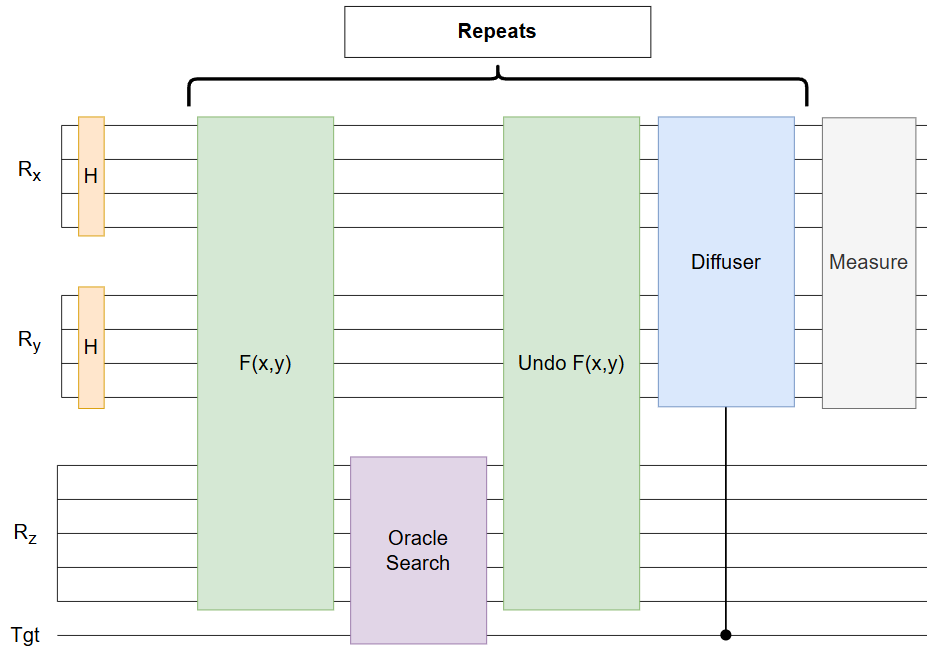
\includegraphics[width=7.9cm]{grover_inversion.png}
  \caption{General circuit diagram for Grover's Algorithm, used to find 
  the inputs $x, y$ for which $f(x,y)=z$, for some known $z$.}
  \label{FIGURA1}
  \end{figure}

  Include one figure showing the oracle, and one figure showing the diffuser.

  \subsection{Semiclassical Arithmetic} 

  Describe our original approach- bitwise addition, registers, operations, etc.

  Mention why an alternative approach was needed.

  Include a drawing of the circuit.

  \subsection{Arithmetic in the Quantum Fourier Domain}  

  Describe the updated methods of quantum arithmetic, and how it solved the 
  previous problems.

  Figures to visualize how the weighted phase shifts work to produce
  expected results matching addition, scaled addition, and register 
  multiplication.

\section{Results and Discussion}

Include some charts showing our runtime and qubit requirements vs N.

  \subsection{Accuracy and Limitations}

  How precise and accurate were our measurements. Mention edge-cases like
  square semiprimes, etc.

  How many qubits were we able to simulate, i.e., how large of semiprimes
  can we factor with our current systems.

  \subsection{Comparison to Shor's Algorithm}

  List strengths and weaknesses of Shor's, i.e., more documentation, more
  examples, larger code base to reference, but ours is faster and uses less
  qubits.

\section{Conclusion}

What have we learned so far, what does it mean, at what problem scale might
we see quantum advantage based on our results, etc.

\section{Future Work}
 
Implementation of the optimization with M, S, p, and q, rather than just 
a and b from N.

\balance

\section*{Acknowledgments}  
% This section is not numbered.
% 
Acknowledge the source paper.


% LateX generates the ``References'' heading automatically and switches
% to 9 point type for the bibliography.  Please  use BibTeX and
% follow the examples in the sample 'refs.bib' file to enter your references.
\bibliography{refs}

% If you don't use BibTeX (why not?) , comment out or remove the previous
% line, and uncomment the following lines up to the ``}\end{bibliography}''
% line below:
%\begin{thebibliography}{99}{ %\small
% \bibitem{tag} (General form) J. K. Author, ``Name of paper,''
%   \emph{Abbrev. Title of
%   Periodical}, vol. x, no. x, pp. xxx--xxx, Abbrev. Month, year. 

% \bibitem{ito}  M. Ito et al., ``Application of amorphous oxide TFT to
%   electrophoretic display,'' \emph{J. Non-Cryst. Solids}, vol. 354, no. 19,
%   pp. 2777--2782, Feb. 2008.
  
% \bibitem{fardel}  R. Fardel, M. Nagel, F. Nuesch, T. Lippert, and
%   A. Wokaun, ``Fabrication of organic light emitting diode pixels by
%   laser-assisted forward transfer,'' \emph{Appl. Phys. Lett.}, vol. 91,
%   no. 6, Aug. 2007, Art. no. 061103.
  
% \bibitem{buncombe} J. U. Buncombe, ``Infrared navigation Part I: Theory,''
%     \emph{IEEE Trans. Aerosp. Electron. Syst.}, vol. AES-4, no. 3,
%     pp. 352--377, Sep. 1944.
      
% Uncomment the following line if you are not using BibTeX.
%}\end{thebibliography}


% LaTeX inserts the ``Address for correspondence'' heading.
\begin{correspondence}
Jacob Collins\\
1565 Filbert Ave\\
jbcollins@csuchico.edu
\end{correspondence}

\end{document}

